\subsection{PageRank: Complejidad}

En el caso de PageRank, la complejidad del algoritmo esta dictada por el tamaño del grafo que representa la red, con lo cual vamos a estudiar el tiempo de ejecución en función de dicho factor.

Para generar las instancias tomamos igual cantidad de nodos y de ejes, la primera tomando valor 30, cada instancia sucesiva aumentamos la cantidad de nodos en 15, hasta llegar a las 150 iteraciones. Esto lo hacemos utilizando un $\alpha = 0.85$ como factor de teletransportacion y un $\epsilon = 10^{-5}$ como factor de convergencia. En la matriz el tamaño esta dado en función de la cantidad de nodos, mientras que los ejes son utilizados en el paso inicial para determinar las probablidades iniciales, con lo cual la cantidad de ejes no tiene la misma importancia que la cantidad de nodos al calcular el método de la potencia.

El siguiente gráfico muestra los tiempos de convergencia según el tamaño, para suavizar el ruido se tomaron 5 muestras por cada instancia y se luego tomo el promedio.

\begin{figure}[H]
\centering
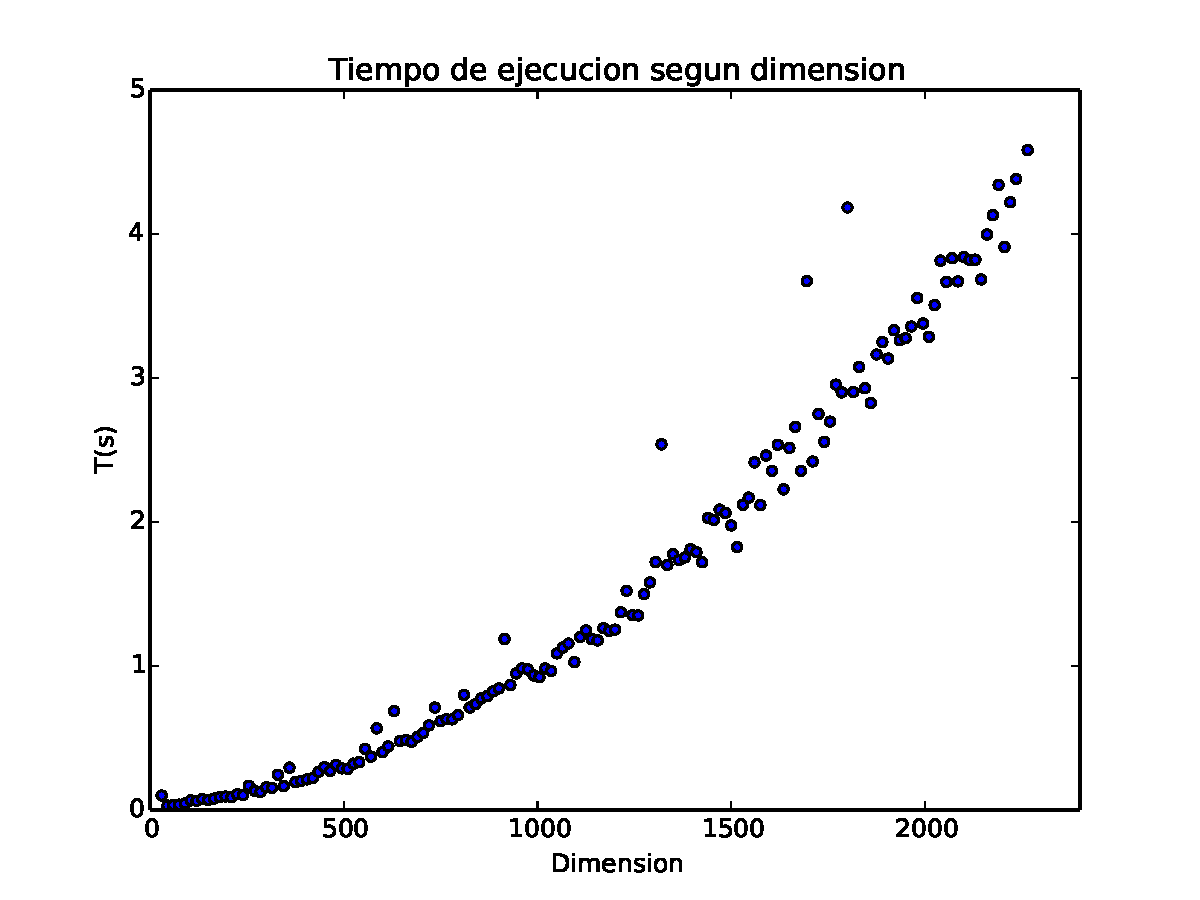
\includegraphics[scale=0.7]{images/complejidad.pdf}
\caption{Tiempos de ejecución según cantidad de webs.}
\label{timePageRank}
\end{figure}

El método de la potencia hace $k$ productos de matrices en \order{n^3}, donde $k$ es la cantidad de iteraciones que toma cada instancia en converger y $n$ es la cantidad de vértices del grafo. Como podemos observar, la tendencia es no lineal. Esto tiene sentido, dado que el producto de matrices es de orden cubico. Luego experimentaremos para ver si la dimension del grafo efectivamente tiene un gran impacto sobre la cantidad de iteraciones que necesita el método para converger. Sin embargo, a priori conjeturamos que la tendencia cubica de este gráfico esta dominada por el orden del producto entre matrices.